% Options for packages loaded elsewhere
\PassOptionsToPackage{unicode}{hyperref}
\PassOptionsToPackage{hyphens}{url}
%
\documentclass[
  ignorenonframetext,
]{beamer}
\usepackage{pgfpages}
\setbeamertemplate{caption}[numbered]
\setbeamertemplate{caption label separator}{: }
\setbeamercolor{caption name}{fg=normal text.fg}
\beamertemplatenavigationsymbolsempty
% Prevent slide breaks in the middle of a paragraph
\widowpenalties 1 10000
\raggedbottom
\setbeamertemplate{part page}{
  \centering
  \begin{beamercolorbox}[sep=16pt,center]{part title}
    \usebeamerfont{part title}\insertpart\par
  \end{beamercolorbox}
}
\setbeamertemplate{section page}{
  \centering
  \begin{beamercolorbox}[sep=12pt,center]{part title}
    \usebeamerfont{section title}\insertsection\par
  \end{beamercolorbox}
}
\setbeamertemplate{subsection page}{
  \centering
  \begin{beamercolorbox}[sep=8pt,center]{part title}
    \usebeamerfont{subsection title}\insertsubsection\par
  \end{beamercolorbox}
}
\AtBeginPart{
  \frame{\partpage}
}
\AtBeginSection{
  \ifbibliography
  \else
    \frame{\sectionpage}
  \fi
}
\AtBeginSubsection{
  \frame{\subsectionpage}
}
\usepackage{amsmath,amssymb}
\usepackage{lmodern}
\usepackage{iftex}
\ifPDFTeX
  \usepackage[T1]{fontenc}
  \usepackage[utf8]{inputenc}
  \usepackage{textcomp} % provide euro and other symbols
\else % if luatex or xetex
  \usepackage{unicode-math}
  \defaultfontfeatures{Scale=MatchLowercase}
  \defaultfontfeatures[\rmfamily]{Ligatures=TeX,Scale=1}
\fi
\usetheme[]{Ilmenau}
% Use upquote if available, for straight quotes in verbatim environments
\IfFileExists{upquote.sty}{\usepackage{upquote}}{}
\IfFileExists{microtype.sty}{% use microtype if available
  \usepackage[]{microtype}
  \UseMicrotypeSet[protrusion]{basicmath} % disable protrusion for tt fonts
}{}
\makeatletter
\@ifundefined{KOMAClassName}{% if non-KOMA class
  \IfFileExists{parskip.sty}{%
    \usepackage{parskip}
  }{% else
    \setlength{\parindent}{0pt}
    \setlength{\parskip}{6pt plus 2pt minus 1pt}}
}{% if KOMA class
  \KOMAoptions{parskip=half}}
\makeatother
\usepackage{xcolor}
\newif\ifbibliography
\usepackage{color}
\usepackage{fancyvrb}
\newcommand{\VerbBar}{|}
\newcommand{\VERB}{\Verb[commandchars=\\\{\}]}
\DefineVerbatimEnvironment{Highlighting}{Verbatim}{commandchars=\\\{\}}
% Add ',fontsize=\small' for more characters per line
\usepackage{framed}
\definecolor{shadecolor}{RGB}{248,248,248}
\newenvironment{Shaded}{\begin{snugshade}}{\end{snugshade}}
\newcommand{\AlertTok}[1]{\textcolor[rgb]{0.94,0.16,0.16}{#1}}
\newcommand{\AnnotationTok}[1]{\textcolor[rgb]{0.56,0.35,0.01}{\textbf{\textit{#1}}}}
\newcommand{\AttributeTok}[1]{\textcolor[rgb]{0.77,0.63,0.00}{#1}}
\newcommand{\BaseNTok}[1]{\textcolor[rgb]{0.00,0.00,0.81}{#1}}
\newcommand{\BuiltInTok}[1]{#1}
\newcommand{\CharTok}[1]{\textcolor[rgb]{0.31,0.60,0.02}{#1}}
\newcommand{\CommentTok}[1]{\textcolor[rgb]{0.56,0.35,0.01}{\textit{#1}}}
\newcommand{\CommentVarTok}[1]{\textcolor[rgb]{0.56,0.35,0.01}{\textbf{\textit{#1}}}}
\newcommand{\ConstantTok}[1]{\textcolor[rgb]{0.00,0.00,0.00}{#1}}
\newcommand{\ControlFlowTok}[1]{\textcolor[rgb]{0.13,0.29,0.53}{\textbf{#1}}}
\newcommand{\DataTypeTok}[1]{\textcolor[rgb]{0.13,0.29,0.53}{#1}}
\newcommand{\DecValTok}[1]{\textcolor[rgb]{0.00,0.00,0.81}{#1}}
\newcommand{\DocumentationTok}[1]{\textcolor[rgb]{0.56,0.35,0.01}{\textbf{\textit{#1}}}}
\newcommand{\ErrorTok}[1]{\textcolor[rgb]{0.64,0.00,0.00}{\textbf{#1}}}
\newcommand{\ExtensionTok}[1]{#1}
\newcommand{\FloatTok}[1]{\textcolor[rgb]{0.00,0.00,0.81}{#1}}
\newcommand{\FunctionTok}[1]{\textcolor[rgb]{0.00,0.00,0.00}{#1}}
\newcommand{\ImportTok}[1]{#1}
\newcommand{\InformationTok}[1]{\textcolor[rgb]{0.56,0.35,0.01}{\textbf{\textit{#1}}}}
\newcommand{\KeywordTok}[1]{\textcolor[rgb]{0.13,0.29,0.53}{\textbf{#1}}}
\newcommand{\NormalTok}[1]{#1}
\newcommand{\OperatorTok}[1]{\textcolor[rgb]{0.81,0.36,0.00}{\textbf{#1}}}
\newcommand{\OtherTok}[1]{\textcolor[rgb]{0.56,0.35,0.01}{#1}}
\newcommand{\PreprocessorTok}[1]{\textcolor[rgb]{0.56,0.35,0.01}{\textit{#1}}}
\newcommand{\RegionMarkerTok}[1]{#1}
\newcommand{\SpecialCharTok}[1]{\textcolor[rgb]{0.00,0.00,0.00}{#1}}
\newcommand{\SpecialStringTok}[1]{\textcolor[rgb]{0.31,0.60,0.02}{#1}}
\newcommand{\StringTok}[1]{\textcolor[rgb]{0.31,0.60,0.02}{#1}}
\newcommand{\VariableTok}[1]{\textcolor[rgb]{0.00,0.00,0.00}{#1}}
\newcommand{\VerbatimStringTok}[1]{\textcolor[rgb]{0.31,0.60,0.02}{#1}}
\newcommand{\WarningTok}[1]{\textcolor[rgb]{0.56,0.35,0.01}{\textbf{\textit{#1}}}}
\setlength{\emergencystretch}{3em} % prevent overfull lines
\providecommand{\tightlist}{%
  \setlength{\itemsep}{0pt}\setlength{\parskip}{0pt}}
\setcounter{secnumdepth}{-\maxdimen} % remove section numbering
\setbeamertemplate{navigation symbols}{}
\setbeamertemplate{footline}[page number]
\usepackage{amsmath}
\ifLuaTeX
  \usepackage{selnolig}  % disable illegal ligatures
\fi
\IfFileExists{bookmark.sty}{\usepackage{bookmark}}{\usepackage{hyperref}}
\IfFileExists{xurl.sty}{\usepackage{xurl}}{} % add URL line breaks if available
\urlstyle{same} % disable monospaced font for URLs
\hypersetup{
  pdftitle={Multivariate Analysis Lecture 7: Hotelling's T2},
  hidelinks,
  pdfcreator={LaTeX via pandoc}}

\title{Multivariate Analysis Lecture 7: Hotelling's T2}
\author{Zhaoxia Yu\\
Professor, Department of Statistics}
\date{2023-04-26}

\begin{document}
\frame{\titlepage}

\begin{frame}{Outline of Lecture 07}
\protect\hypertarget{outline-of-lecture-07}{}
\begin{itemize}
\tightlist
\item
  Review of Wishart and the Hotelling's \(T^2\) distribution for
  one-sample problems
\item
  Examples of one-sample Hotelling's \(T^2\)
\item
  Two-sample Hotelling's \(T^2\)
\item
  Examples of two-sample Hotelling's \(T^2\)
\item
  The multivariate normality (MVN) assumption
\end{itemize}
\end{frame}

\hypertarget{review}{%
\section{Review}\label{review}}

\hypertarget{wishart-distribution}{%
\subsection{Wishart Distribution}\label{wishart-distribution}}

\begin{frame}{Definition of Wishart Distribution}
\protect\hypertarget{definition-of-wishart-distribution}{}
\begin{itemize}
\item
  A Wishart distribution can be defined in the following way
\item
  Let \(\mathbf W\) be a \(p\times p\) random matrix. We say
  \(\mathbf W\) follows \(Wishart_{p}(k, \boldsymbol \Sigma)\) if
  \(\mathbf W\) can be written as \(\mathbf W=\mathbf X^T \mathbf X\)
  where \(\mathbf X\) denotes the random matrix formed by a random
  sample of size \(k\) from MVN \(N(\mathbf 0, \boldsymbol \Sigma)\).
\item
  The definition indicates that if we have a random sample
  \(\mathbf X_1, \cdots \mathbf X_k\) from
  \(N(\mathbf 0, \boldsymbol \Sigma)\), then
  \(\mathbf X^T \mathbf X=\sum_{i=1}^k \mathbf X_i \mathbf X_i^T \sim Wishart_p(k, \boldsymbol \Sigma)\).
\item
  Remark:\(E[\mathbf W]=k\Sigma\).
\end{itemize}
\end{frame}

\begin{frame}{Wishart vs Chi-squared}
\protect\hypertarget{wishart-vs-chi-squared}{}
\begin{itemize}
\item
  \textcolor{red}{Wishart}: If
  \(\mathbf X_1, \cdots \mathbf X_k \overset{iid}\sim N(\mathbf 0, \boldsymbol \Sigma)\),
  then
  \[\mathbf X^T \mathbf X =\sum_{i=1}^k \mathbf X_i\mathbf X_i^T \sim Wishart_p(k, \boldsymbol \Sigma) \mbox{, where } \mathbf X_{k\times p}=\begin{pmatrix}
  X_1^T\\ \vdots\\ X_k^T
  \end{pmatrix}
  \]
\item
  \textcolor{red}{Chi-squared}: If
  \(X_1, \cdots, X_k \overset{iid}\sim N(0,1)\), then\\
  \[\mathbf X^T\mathbf X=\sum_{i=1}^k X_i^2\sim \chi_k^2 \mbox{, where } \mathbf X_{k\times 1}= 
  \begin{pmatrix}
  X_1 \\ \vdots \\ X_k
  \end{pmatrix}\]
\end{itemize}
\end{frame}

\begin{frame}{Wishart vs Chi-squared (continued)}
\protect\hypertarget{wishart-vs-chi-squared-continued}{}
\begin{itemize}
\tightlist
\item
  When \(p=1\),
  \[W=\sum_{i=1}^k X_i^2 = \sigma^2 \sum_{i=1}^k \left(\frac{X_i}{\sigma} \right)^2\sim \sigma^2 \chi_k^2 \]
\end{itemize}
\end{frame}

\begin{frame}{The Sample Covariance Matrix}
\protect\hypertarget{the-sample-covariance-matrix}{}
\begin{itemize}
\item
  Let \(\mathbf X_1, \cdots \mathbf X_n\) be a random sample from
  \(N(\boldsymbol \mu, \boldsymbol \Sigma)\). The
  \(\mathbf X_{n\times p}\) follows a matrix normal distribution:
  \[\mathbf X \sim N(\mathbf 1_n \otimes \boldsymbol \mu^T, \boldsymbol \Sigma, \mathbf I_n)\]
\item
  We have shown that
\end{itemize}

\[(n-1)\mathbf S \sim Wishart_p(n-1, \boldsymbol\Sigma)\]
\end{frame}

\hypertarget{hotellings-t2}{%
\subsection{\texorpdfstring{Hotelling's
\(T^2\)}{Hotelling's T\^{}2}}\label{hotellings-t2}}

\begin{frame}{Definition of Hotelling's \(T^2\)}
\protect\hypertarget{definition-of-hotellings-t2}{}
\begin{itemize}
\tightlist
\item
  Hotelling generalized the student's t, which is for univarite, to
  Hotelling's T2, which is the multivariate version
\item
  \textcolor{red}{Definition. }We say a random variable follows
  Hotelling's \(T_{p,\nu}^2\) if the random variable can be written as
  \(\mathbf Z^T\left(\frac{W}{\nu}\right)^{-1}\mathbf Z\) where

  \begin{enumerate}
  \tightlist
  \item
    \(\mathbf Z\sim N(\mathbf 0, \boldsymbol\Sigma)\)
  \item
    \(\mathbf W \sim W_p(\nu, \boldsymbol\Sigma)\)
  \item
    \(\mathbf Z \perp \mathbf W\)
  \end{enumerate}
\end{itemize}
\end{frame}

\hypertarget{one-sample-hotelling-t2}{%
\section{\texorpdfstring{One-Sample Hotelling
\(T^2\)}{One-Sample Hotelling T\^{}2}}\label{one-sample-hotelling-t2}}

\begin{frame}{One-Sample Hotelling \(T^2\)}
\protect\hypertarget{one-sample-hotelling-t2-1}{}
\begin{itemize}
\item
  Let \(\boldsymbol{X}_1, \boldsymbol{X}_2, ..., \boldsymbol{X}_n\) be a
  random sample from a multivariate normal distribution with mean vector
  \(\boldsymbol{\mu}\) and covariance matrix \(\boldsymbol{\Sigma}\).
\item
  The sample mean vector and sample covariance matrix are denoted by
  \(\bar{\mathbf X}\) and \(\mathbf S\), respectively.
\item
  The null hypothesis of interest
  \(H_0: \boldsymbol \mu = \boldsymbol \mu_0\)
\item
  The one-sample Hotelling \(T^2\) is defined as
  \[T^2=(\hat{\mathbf \mu} - \mathbf \mu_0)^T \left(Cov(\hat{\mathbf \mu})\right)^{-1}(\hat{\mathbf \mu} - \mathbf \mu_0)\]
\item
  We have shown that \(T^2\sim T_{p, n-1}^2\) when
  \(H_0: \boldsymbol \mu=\boldsymbol \mu_0\).
\end{itemize}
\end{frame}

\begin{frame}{Hotelling's \(T^2\) Distribution vs \(F\) Distribution}
\protect\hypertarget{hotellings-t2-distribution-vs-f-distribution}{}
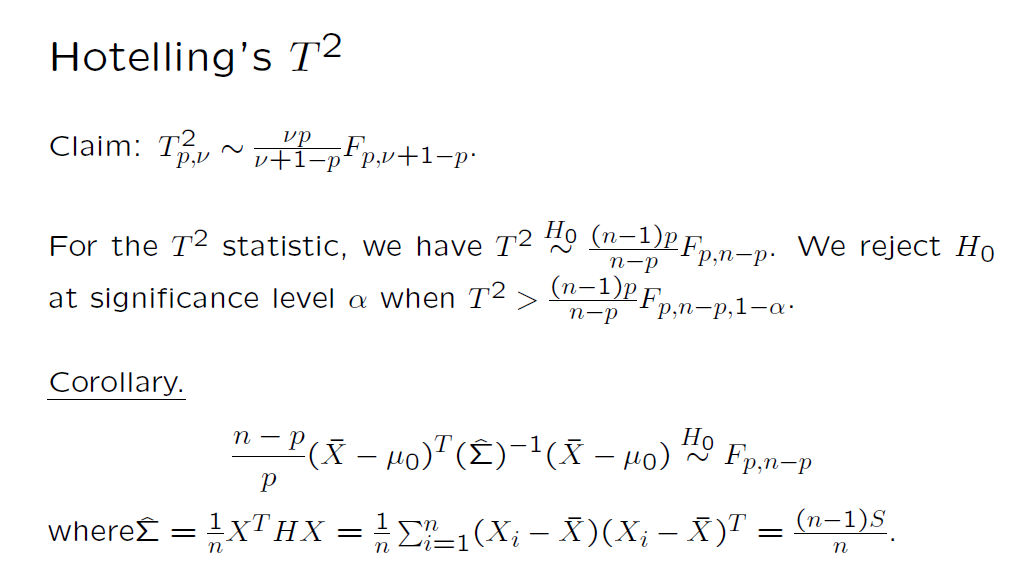
\includegraphics[width=0.8\linewidth]{img/T2vsF}
\end{frame}

\hypertarget{a-simulation-study}{%
\subsection{A Simulation Study}\label{a-simulation-study}}

\begin{frame}[fragile]{Understand the Wishart Distribution}
\protect\hypertarget{understand-the-wishart-distribution}{}
\begin{itemize}
\tightlist
\item
  Recall that if \(W\sim Wishart_p(k, \boldsymbol \Sigma)\), then
  \(E[\mathbf W]=k\Sigma\).
\end{itemize}

\tiny

\begin{Shaded}
\begin{Highlighting}[]
\FunctionTok{library}\NormalTok{(MASS)}
\NormalTok{p}\OtherTok{=}\DecValTok{2}\NormalTok{; n}\OtherTok{=}\DecValTok{5}\NormalTok{; B}\OtherTok{=}\DecValTok{1000}\NormalTok{; rho}\OtherTok{=}\FloatTok{0.7}
\NormalTok{Sigma}\OtherTok{=}\FunctionTok{diag}\NormalTok{(}\DecValTok{1}\SpecialCharTok{+}\NormalTok{rho, p, p) }\SpecialCharTok{{-}} \FunctionTok{matrix}\NormalTok{(rho, p, p)}
\NormalTok{wmat.array}\OtherTok{=}\FunctionTok{array}\NormalTok{(}\DecValTok{0}\NormalTok{, }\FunctionTok{c}\NormalTok{(B, p, p)) }\CommentTok{\#wishart{-}distributed}
\ControlFlowTok{for}\NormalTok{(b }\ControlFlowTok{in} \DecValTok{1}\SpecialCharTok{:}\NormalTok{B)\{}
\NormalTok{  X}\OtherTok{=}\FunctionTok{mvrnorm}\NormalTok{(n, }\FunctionTok{rep}\NormalTok{(}\DecValTok{0}\NormalTok{,p), Sigma)}
\NormalTok{  wmat.array[b,,]}\OtherTok{=}\FunctionTok{cov}\NormalTok{(X)\}}
\FunctionTok{apply}\NormalTok{(wmat.array, }\FunctionTok{c}\NormalTok{(}\DecValTok{2}\NormalTok{,}\DecValTok{3}\NormalTok{), mean)}
\end{Highlighting}
\end{Shaded}

\begin{verbatim}
##            [,1]       [,2]
## [1,]  0.9968851 -0.6949237
## [2,] -0.6949237  1.0046583
\end{verbatim}

\begin{Shaded}
\begin{Highlighting}[]
\NormalTok{Sigma}\SpecialCharTok{*}\NormalTok{(n}\DecValTok{{-}1}\NormalTok{)}
\end{Highlighting}
\end{Shaded}

\begin{verbatim}
##      [,1] [,2]
## [1,]  4.0 -2.8
## [2,] -2.8  4.0
\end{verbatim}

\normalsize
\end{frame}

\begin{frame}[fragile]{Write an R function to conduct Hotelling's
\(T^2\)}
\protect\hypertarget{write-an-r-function-to-conduct-hotellings-t2}{}
\begin{itemize}
\tightlist
\item
  There is no R base function for conducting Hotelling's \(T^2\) test
\item
  We will write an R function
\end{itemize}

\tiny

\begin{Shaded}
\begin{Highlighting}[]
\CommentTok{\#Hotelling\textquotesingle{}s T\^{}2 for testing H0: mu=mu0 vs mu != mu0}
\NormalTok{Hotelling.T2}\FloatTok{.1}\NormalTok{sample}\OtherTok{=}\ControlFlowTok{function}\NormalTok{(X, mu0)}
\NormalTok{\{}
\NormalTok{  n}\OtherTok{=}\FunctionTok{dim}\NormalTok{(X)[}\DecValTok{1}\NormalTok{]}
\NormalTok{  p}\OtherTok{=}\FunctionTok{dim}\NormalTok{(X)[}\DecValTok{2}\NormalTok{]}
\NormalTok{  X.bar}\OtherTok{=}\FunctionTok{colMeans}\NormalTok{(X)}
\NormalTok{  X.S}\OtherTok{=}\FunctionTok{cov}\NormalTok{(X)}
\NormalTok{  T2}\OtherTok{=}\NormalTok{n}\SpecialCharTok{*}\FunctionTok{t}\NormalTok{(X.bar}\SpecialCharTok{{-}}\NormalTok{mu0)}\SpecialCharTok{\%*\%}\FunctionTok{solve}\NormalTok{(X.S)}\SpecialCharTok{\%*\%}\NormalTok{(X.bar}\SpecialCharTok{{-}}\NormalTok{mu0)}
\NormalTok{  p.value}\OtherTok{=}\DecValTok{1}\SpecialCharTok{{-}}\FunctionTok{pf}\NormalTok{(T2}\SpecialCharTok{/}\NormalTok{((n}\DecValTok{{-}1}\NormalTok{)}\SpecialCharTok{*}\NormalTok{p}\SpecialCharTok{/}\NormalTok{(n}\SpecialCharTok{{-}}\NormalTok{p)),p,n}\SpecialCharTok{{-}}\NormalTok{p)}
  \FunctionTok{return}\NormalTok{(}\FunctionTok{list}\NormalTok{(}\AttributeTok{X.bar=}\NormalTok{X.bar, }\AttributeTok{X.cov=}\NormalTok{X.S, }\AttributeTok{T2=}\NormalTok{T2, }\AttributeTok{p.value=}\NormalTok{p.value))}
\NormalTok{\}}
\end{Highlighting}
\end{Shaded}

\normalsize
\end{frame}

\begin{frame}[fragile]{Example of Multivariate One-Sample Problem:
Protein Intake}
\protect\hypertarget{example-of-multivariate-one-sample-problem-protein-intake}{}
\begin{itemize}
\tightlist
\item
  For the protein intake data, it might be more interesting to estimate
  the means than conducting hypothesis testing
\item
  Suppose we are interested in estimating the means of the daily protein
  intake from different sources
\end{itemize}

\tiny

\begin{Shaded}
\begin{Highlighting}[]
\FunctionTok{library}\NormalTok{(MASS)}\CommentTok{\#the library "MASS" is required}
\NormalTok{my.cov}\OtherTok{=}\DecValTok{4}\SpecialCharTok{*}\NormalTok{(}\FunctionTok{diag}\NormalTok{(}\DecValTok{4}\NormalTok{) }\SpecialCharTok{+} \FloatTok{0.3}\SpecialCharTok{*} \FunctionTok{rep}\NormalTok{(}\DecValTok{1}\NormalTok{,}\DecValTok{4}\NormalTok{)}\SpecialCharTok{\%o\%}\FunctionTok{rep}\NormalTok{(}\DecValTok{1}\NormalTok{,}\DecValTok{4}\NormalTok{))}
\NormalTok{n}\OtherTok{=}\DecValTok{60}\NormalTok{;p}\OtherTok{=}\DecValTok{4}
\NormalTok{my.mean}\OtherTok{=}\DecValTok{8}\SpecialCharTok{*}\FunctionTok{c}\NormalTok{(}\DecValTok{3}\NormalTok{,}\DecValTok{2}\NormalTok{,}\DecValTok{1}\NormalTok{,}\DecValTok{1}\NormalTok{)}
\FunctionTok{eigen}\NormalTok{(my.cov)}\CommentTok{\#to check whether the cov matrix is p.d.}
\end{Highlighting}
\end{Shaded}

\begin{verbatim}
## eigen() decomposition
## $values
## [1] 8.8 4.0 4.0 4.0
## 
## $vectors
##      [,1]       [,2]       [,3]       [,4]
## [1,] -0.5  0.8660254  0.0000000  0.0000000
## [2,] -0.5 -0.2886751 -0.5773503 -0.5773503
## [3,] -0.5 -0.2886751 -0.2113249  0.7886751
## [4,] -0.5 -0.2886751  0.7886751 -0.2113249
\end{verbatim}

\normalsize
\end{frame}

\begin{frame}[fragile]{Example of Multivariate One-Sample Problem:
Protein Intake}
\protect\hypertarget{example-of-multivariate-one-sample-problem-protein-intake-1}{}
\begin{itemize}
\tightlist
\item
  Estimate the mean vector using the sample mean vector
\item
  Estimate covariance of the sample mean vector. Recall that
  \(cov(\bar{\mathbf X})=\frac{\boldsymbol \Sigma}{n}\)
\end{itemize}

\tiny

\begin{Shaded}
\begin{Highlighting}[]
\FunctionTok{set.seed}\NormalTok{(}\DecValTok{1}\NormalTok{)}
\NormalTok{x}\OtherTok{=}\FunctionTok{mvrnorm}\NormalTok{(n, }\AttributeTok{mu=}\NormalTok{my.mean, }\AttributeTok{Sigma=}\NormalTok{my.cov)}
\NormalTok{protein}\OtherTok{=}\FunctionTok{as.matrix}\NormalTok{(}\FunctionTok{data.frame}\NormalTok{(}\AttributeTok{meat=}\NormalTok{x[,}\DecValTok{1}\NormalTok{],}\AttributeTok{dairy=}\NormalTok{x[,}\DecValTok{2}\NormalTok{], }
                             \AttributeTok{veg=}\NormalTok{x[,}\DecValTok{3}\NormalTok{], }\AttributeTok{other=}\NormalTok{x[,}\DecValTok{4}\NormalTok{]))}
\FunctionTok{colMeans}\NormalTok{(protein)}
\end{Highlighting}
\end{Shaded}

\begin{verbatim}
##      meat     dairy       veg     other 
## 24.034032 15.928361  7.660490  7.738634
\end{verbatim}

\begin{Shaded}
\begin{Highlighting}[]
\FunctionTok{cov}\NormalTok{(protein)}\SpecialCharTok{/}\NormalTok{n}
\end{Highlighting}
\end{Shaded}

\begin{verbatim}
##             meat       dairy         veg       other
## meat  0.07159404 0.013584596 0.018824131 0.009220700
## dairy 0.01358460 0.073421655 0.005829816 0.003895500
## veg   0.01882413 0.005829816 0.086176323 0.009828535
## other 0.00922070 0.003895500 0.009828535 0.075478822
\end{verbatim}

\normalsize
\end{frame}

\begin{frame}{Example of Multivariate One-Sample Problem: Protein
Intake}
\protect\hypertarget{example-of-multivariate-one-sample-problem-protein-intake-2}{}
\begin{itemize}
\tightlist
\item
  Use Hotelling's \(T^2\) to quantify uncertainties. Recall that
  \[T^2=(\bar{\mathbf X} - \boldsymbol \mu)^T \left(Cov(\bar{\mathbf X})\right)^{-1}(\bar{\mathbf X} - \boldsymbol \mu)\sim \frac{(n-1)p}{n-p} F_{p, n-p}\]
\end{itemize}

where \(Cov(\bar{\mathbf X})=\frac{\mathbf S}{n}\).

\begin{itemize}
\item
  The result indicates that
  \[Pr[(\bar{\mathbf X} - \boldsymbol \mu)^T \left(Cov(\bar{\mathbf X})\right)^{-1}(\bar{\mathbf X} - \boldsymbol \mu)\le \frac{(n-1)p}{n-p} F_{p, n-p, 1-\alpha}]=1-\alpha\]
\item
  Thus, a \((1-\alpha)100\%\) confidence \textcolor{red}{region} for
  \(\boldsymbol \mu\) is
  \[\{\mathbf\mu: (\bar{\mathbf X} - \boldsymbol \mu)^T \left(Cov(\bar{\mathbf X})\right)^{-1}(\bar{\mathbf X} - \boldsymbol \mu)\le \frac{(n-1)p}{n-p} F_{p, n-p, 1-\alpha}\}\]
\end{itemize}
\end{frame}

\begin{frame}{Example of Multivariate One-Sample Problem: Protein
Intake}
\protect\hypertarget{example-of-multivariate-one-sample-problem-protein-intake-3}{}
\begin{itemize}
\tightlist
\item
  Confidence intervals, which are in the form of
  \[\mbox{estimate}\pm \mbox{critical value} \times \mbox{standard error}\]\\
  are often preferred
\item
  If there is only one parameter of interest, we can construct a C.I.
  using t-distribution, just as in univariate analysis
\item
  Example. What is the mean protein intake? We have discussed the
  problem in Lecture 04.

  \begin{itemize}
  \tightlist
  \item
    Lecture 04: we constructed a large-sample C.I. by using 1.96 as the
    critical value. (See the protein intake example)
  \item
    This lecture: we construct a C.I. by using
    \(t_{n-1, 1-\frac{\alpha}{2}}\) as the critical value
  \end{itemize}
\end{itemize}

\(\bar{X}_{(j)} \pm t_{n-1, 1- \frac{\alpha}{2}}\sqrt{\frac{s^2_{X_{(j)}}}{n}} \mbox{ for } j=1,\cdots, p\).
\end{frame}

\begin{frame}{Example of Multivariate One-Sample Problem: Protein
Intake}
\protect\hypertarget{example-of-multivariate-one-sample-problem-protein-intake-4}{}
\begin{itemize}
\tightlist
\item
  The confidence region has exactly \((1-\alpha)100\%\) confidence;
  however
\item
  In many situations, we would like to construct confidence intervals
  for multiple parameters
\item
  This is known as simultaneous intervals
\item
  If we use the conventional method to construct individual C.I.s, we
  will have lower than \((1-\alpha)100\%\) confidence to cover all the
  parameters simultaneously
\end{itemize}
\end{frame}

\begin{frame}{Example of Multivariate One-Sample Problem: Protein
Intake}
\protect\hypertarget{example-of-multivariate-one-sample-problem-protein-intake-5}{}
\begin{itemize}
\tightlist
\item
  Some linear algebra result ensures that the following method gives
  \((1-\alpha)100\%\) confidence to cover all linear combinations of the
  parameters (in the form of \(a^T\boldsymbol \mu\)) simultaneously
  \[a^T\bar{\mathbf X}\pm \sqrt{\frac{(n-1)p}{n-p}F_{p, n-p, 1-\alpha}} se(a^T\bar{\mathbf X}) \]
\item
  Example, consider the individual means \(\mu_j, j=1,\cdots, 4\) in the
  protein intake example, the following intervals are \(95\%\)
  simultaneous C.I. for the mean protein intake from the four sources
\end{itemize}
\end{frame}

\begin{frame}[fragile]{Example of Multivariate One-Sample Problem:
Protein Intake}
\protect\hypertarget{example-of-multivariate-one-sample-problem-protein-intake-6}{}
\tiny

\begin{Shaded}
\begin{Highlighting}[]
\CommentTok{\#sample means}
\FunctionTok{colMeans}\NormalTok{(protein)}
\end{Highlighting}
\end{Shaded}

\begin{verbatim}
##      meat     dairy       veg     other 
## 24.034032 15.928361  7.660490  7.738634
\end{verbatim}

\begin{Shaded}
\begin{Highlighting}[]
\CommentTok{\#standard errors}
\FunctionTok{sqrt}\NormalTok{(}\FunctionTok{diag}\NormalTok{(}\FunctionTok{cov}\NormalTok{(protein)}\SpecialCharTok{/}\NormalTok{n))}
\end{Highlighting}
\end{Shaded}

\begin{verbatim}
##      meat     dairy       veg     other 
## 0.2675706 0.2709643 0.2935580 0.2747341
\end{verbatim}

\begin{Shaded}
\begin{Highlighting}[]
\CommentTok{\#critical value based on T2}
\FunctionTok{sqrt}\NormalTok{((n}\DecValTok{{-}1}\NormalTok{)}\SpecialCharTok{*}\NormalTok{p}\SpecialCharTok{/}\NormalTok{(n}\SpecialCharTok{{-}}\NormalTok{p)}\SpecialCharTok{*}\FunctionTok{qf}\NormalTok{(}\FloatTok{0.95}\NormalTok{, p, n}\SpecialCharTok{{-}}\NormalTok{p))}
\end{Highlighting}
\end{Shaded}

\begin{verbatim}
## [1] 3.269537
\end{verbatim}

\begin{Shaded}
\begin{Highlighting}[]
\CommentTok{\#lower bounds}
\NormalTok{low.bound}\OtherTok{=}\FunctionTok{colMeans}\NormalTok{(protein) }\SpecialCharTok{{-}} \FunctionTok{sqrt}\NormalTok{((n}\DecValTok{{-}1}\NormalTok{)}\SpecialCharTok{*}\NormalTok{p}\SpecialCharTok{/}\NormalTok{(n}\SpecialCharTok{{-}}\NormalTok{p)}\SpecialCharTok{*}\FunctionTok{qf}\NormalTok{(}\FloatTok{0.95}\NormalTok{, p, n}\SpecialCharTok{{-}}\NormalTok{p)) }\SpecialCharTok{*}\FunctionTok{sqrt}\NormalTok{(}\FunctionTok{diag}\NormalTok{(}\FunctionTok{cov}\NormalTok{(protein)}\SpecialCharTok{/}\NormalTok{n))}
\CommentTok{\#upper bounds}
\NormalTok{up.bound}\OtherTok{=}\FunctionTok{colMeans}\NormalTok{(protein) }\SpecialCharTok{+} \FunctionTok{sqrt}\NormalTok{((n}\DecValTok{{-}1}\NormalTok{)}\SpecialCharTok{*}\NormalTok{p}\SpecialCharTok{/}\NormalTok{(n}\SpecialCharTok{{-}}\NormalTok{p)}\SpecialCharTok{*}\FunctionTok{qf}\NormalTok{(}\FloatTok{0.95}\NormalTok{, p, n}\SpecialCharTok{{-}}\NormalTok{p)) }\SpecialCharTok{*}\FunctionTok{sqrt}\NormalTok{(}\FunctionTok{diag}\NormalTok{(}\FunctionTok{cov}\NormalTok{(protein)}\SpecialCharTok{/}\NormalTok{n))}
\end{Highlighting}
\end{Shaded}

\normalsize
\end{frame}

\begin{frame}[fragile]{Example of Multivariate One-Sample Problem:
Protein Intake}
\protect\hypertarget{example-of-multivariate-one-sample-problem-protein-intake-7}{}
\begin{Shaded}
\begin{Highlighting}[]
\CommentTok{\#put everything into a table}
\FunctionTok{data.frame}\NormalTok{(}\AttributeTok{lower=}\NormalTok{low.bound, }\AttributeTok{mean=}\FunctionTok{colMeans}\NormalTok{(protein), }
           \AttributeTok{upper=}\NormalTok{up.bound)}
\end{Highlighting}
\end{Shaded}

\begin{verbatim}
##           lower      mean     upper
## meat  23.159200 24.034032 24.908864
## dairy 15.042433 15.928361 16.814289
## veg    6.700691  7.660490  8.620288
## other  6.840381  7.738634  8.636887
\end{verbatim}
\end{frame}

\begin{frame}{Example of Multivariate One-Sample Problem: Protein
Intake}
\protect\hypertarget{example-of-multivariate-one-sample-problem-protein-intake-8}{}
\begin{itemize}
\tightlist
\item
  Three choices of criticl values

  \begin{itemize}
  \tightlist
  \item
    unadjusted: \(t_{n-1, 1-\alpha/2}\). Should \textcolor{red}{NOT} be
    used if multiple linear functions need to be estimated
  \item
    \(T^2\): \(\sqrt{\frac{(n-1)p}{n-p}F_{p, n-p, 1-\alpha}}\)
  \item
    Bonferroni's correction: simply replace \(\alpha\) with \(\alpha/k\)
    where \(k\) is the total number of linear functions of the mean
    parameters: \(t_{n-1, 1-\alpha/(2k)}\)
  \end{itemize}
\item
  Example: the critical values for the individual means from four
  protein sources
\end{itemize}
\end{frame}

\begin{frame}[fragile]{Example of Multivariate One-Sample Problem:
Protein Intake}
\protect\hypertarget{example-of-multivariate-one-sample-problem-protein-intake-9}{}
\tiny

\begin{Shaded}
\begin{Highlighting}[]
\CommentTok{\#unadjusted, shouldn\textquotesingle{}t be used when constructing simultaneous C.I.s}
\FunctionTok{qt}\NormalTok{(}\DecValTok{1}\FloatTok{{-}0.05}\SpecialCharTok{/}\DecValTok{2}\NormalTok{, n}\DecValTok{{-}1}\NormalTok{)}
\end{Highlighting}
\end{Shaded}

\begin{verbatim}
## [1] 2.000995
\end{verbatim}

\begin{Shaded}
\begin{Highlighting}[]
\CommentTok{\#T\^{}2}
\FunctionTok{sqrt}\NormalTok{((n}\DecValTok{{-}1}\NormalTok{)}\SpecialCharTok{*}\NormalTok{p}\SpecialCharTok{/}\NormalTok{(n}\SpecialCharTok{{-}}\NormalTok{p)}\SpecialCharTok{*}\FunctionTok{qf}\NormalTok{(}\FloatTok{0.95}\NormalTok{, p, n}\SpecialCharTok{{-}}\NormalTok{p))}
\end{Highlighting}
\end{Shaded}

\begin{verbatim}
## [1] 3.269537
\end{verbatim}

\begin{Shaded}
\begin{Highlighting}[]
\CommentTok{\#Bonferroni correction}
\FunctionTok{qt}\NormalTok{(}\DecValTok{1}\FloatTok{{-}0.05}\SpecialCharTok{/}\NormalTok{p}\SpecialCharTok{/}\DecValTok{2}\NormalTok{, n}\DecValTok{{-}1}\NormalTok{)}
\end{Highlighting}
\end{Shaded}

\begin{verbatim}
## [1] 2.576588
\end{verbatim}

\normalsize
\end{frame}

\hypertarget{two-sample-hotellings-t2}{%
\section{\texorpdfstring{Two-Sample Hotellings
\(T^2\)}{Two-Sample Hotellings T\^{}2}}\label{two-sample-hotellings-t2}}

\begin{frame}{One-Sample vs Two-Sample}
\protect\hypertarget{one-sample-vs-two-sample}{}
\begin{itemize}
\tightlist
\item
  In the one-sample problem, the goal is to make inference of

  \begin{itemize}
  \tightlist
  \item
    univariate: a population mean (one-sample t-test problem) or
  \item
    multivariate: a population mean vector (one-sample Hotelling \(T^2\)
    problem)
  \end{itemize}
\item
  In the two-sample problem

  \begin{itemize}
  \tightlist
  \item
    univariate: compare two population means
  \item
    multivariate: compare two population mean vectors
  \end{itemize}
\end{itemize}
\end{frame}

\begin{frame}{Univariate Two-Sample Problems}
\protect\hypertarget{univariate-two-sample-problems}{}
\begin{itemize}
\tightlist
\item
  Two independent samples

  \begin{itemize}
  \tightlist
  \item
    Sample 1 is from population 1:
  \end{itemize}

  \[X_{11}, \cdots, X_{1,n_1}\overset{iid} \sim N(\mu_1,\sigma^2)\]

  \begin{itemize}
  \tightlist
  \item
    Sample 2 is from population 2:
  \end{itemize}

  \[X_{21}, \cdots, X_{2,n_2}\overset{iid} \sim N(\mu_2,\sigma^2)\]
\item
  Null hypothesis: \(H_0: \mu_1=\mu_2\)
\end{itemize}
\end{frame}

\begin{frame}{Univariate Two-Sample Problems}
\protect\hypertarget{univariate-two-sample-problems-1}{}
\begin{itemize}
\tightlist
\item
  Pooled sample variance
\end{itemize}

\[s^2_p = \dfrac{(n_1-1)s^2_1+(n_2-1)s^2_2}{n_1+n_2-2}\] where
\[s^2_i = \dfrac{\sum_{j=1}^{n_i}X^2_{ij}-(\sum_{j=1}^{n_i}X_{ij})^2/n_i}{n_i-1}\]

\begin{itemize}
\item
  Two-sample t-statistic
  \[t = \dfrac{\bar{x}_1-\bar{x}_2}{\sqrt{s^2_p(\dfrac{1}{n_1}+\dfrac{1}{n_2})}} \]
\item
  Null distribution: \(t\overset{H_0}\sim t_{n_1+n_2-2}\).
\end{itemize}
\end{frame}

\begin{frame}{Multivarite Two-Sample Problems}
\protect\hypertarget{multivarite-two-sample-problems}{}
\begin{itemize}
\item
  Two independent samples

  \begin{itemize}
  \tightlist
  \item
    Sample 1 is from population 1:
  \end{itemize}

  \[\mathbf X_{11}, \cdots,\mathbf  X_{1,n_1}\overset{iid} \sim N(\boldsymbol \mu_1, \boldsymbol \Sigma)\]

  \begin{itemize}
  \tightlist
  \item
    Sample 2 is from population 2:
  \end{itemize}

  \[\mathbf X_{21}, \cdots,\mathbf  X_{2,n_2}\overset{iid} \sim N(\boldsymbol \mu_2, \boldsymbol \Sigma)\]
\item
  Null and alternative hypotheses:
  \(H_0: \boldsymbol \mu_1=\boldsymbol \mu_2\) vs
  \(H_1: \boldsymbol \mu_1\not=\boldsymbol \mu_2\)
\end{itemize}
\end{frame}

\begin{frame}{Multivarite Two-Sample Problems}
\protect\hypertarget{multivarite-two-sample-problems-1}{}
\begin{itemize}
\item
  Pooled sample covariance matrix
  \[\mathbf{S}_p = \dfrac{(n_1-1)\mathbf{S}_1+(n_2-1)\mathbf{S}_2}{n_1+n_2-2}\]
  where
  \[\mathbf{S}_i = \dfrac{1}{n_i-1}\sum_{j=1}^{n_i}{(\mathbf X_{ij}-\bar{\mathbf X}_i)(\mathbf X_{ij}-\bar{\mathbf X}_i)'}\]
\item
  Two-sample Hotelling's \(T^2\)
  \[T^2 = {(\bar{\mathbf X}_1 - \bar{\mathbf X}_2)}^T\{\mathbf{S}_p(\frac{1}{n_1}+\frac{1}{n_2})\}^{-1} {(\bar{\mathbf X}_1 - \bar{\mathbf X}_2)}\]
\item
  Null distribution:
  \[T^2 \overset{H_0}\sim \frac{(n_1+n_2-2)p}{n_1+n_2-p-1} F_{p, n_1+n_2-p-1}\]
\end{itemize}
\end{frame}

\begin{frame}[fragile]{Multivariate Two-Sample Problems: Write an R
Function}
\protect\hypertarget{multivariate-two-sample-problems-write-an-r-function}{}
\begin{itemize}
\tightlist
\item
  No existing base function in R.
\end{itemize}

\tiny

\begin{Shaded}
\begin{Highlighting}[]
\NormalTok{Hotelling.T2}\FloatTok{.2}\NormalTok{sample}\OtherTok{=}\ControlFlowTok{function}\NormalTok{(X, Y)\{}
\NormalTok{  n}\OtherTok{=}\FunctionTok{dim}\NormalTok{(X)[}\DecValTok{1}\NormalTok{]; m}\OtherTok{=}\FunctionTok{dim}\NormalTok{(Y)[}\DecValTok{1}\NormalTok{]; p}\OtherTok{=}\FunctionTok{dim}\NormalTok{(X)[}\DecValTok{2}\NormalTok{]}
  \ControlFlowTok{if}\NormalTok{(p}\SpecialCharTok{!=} \FunctionTok{dim}\NormalTok{(Y)[}\DecValTok{2}\NormalTok{]) }\FunctionTok{return}\NormalTok{(}\StringTok{"Error: the dimensions of X and Y are not the same"}\NormalTok{)}
\NormalTok{  X.bar}\OtherTok{=}\FunctionTok{colMeans}\NormalTok{(X); Y.bar}\OtherTok{=}\FunctionTok{colMeans}\NormalTok{(Y)}
\NormalTok{  X.S}\OtherTok{=}\FunctionTok{cov}\NormalTok{(X); Y.S}\OtherTok{=}\FunctionTok{cov}\NormalTok{(Y)}
\NormalTok{  pooled.S}\OtherTok{=}\NormalTok{((n}\DecValTok{{-}1}\NormalTok{)}\SpecialCharTok{*}\NormalTok{X.S}\SpecialCharTok{+}\NormalTok{(m}\DecValTok{{-}1}\NormalTok{)}\SpecialCharTok{*}\NormalTok{Y.S)}\SpecialCharTok{/}\NormalTok{(m}\SpecialCharTok{+}\NormalTok{n}\DecValTok{{-}2}\NormalTok{)}
\NormalTok{  T2}\OtherTok{=}\FunctionTok{t}\NormalTok{(X.bar}\SpecialCharTok{{-}}\NormalTok{Y.bar)}\SpecialCharTok{\%*\%}\FunctionTok{solve}\NormalTok{((}\DecValTok{1}\SpecialCharTok{/}\NormalTok{n}\SpecialCharTok{+}\DecValTok{1}\SpecialCharTok{/}\NormalTok{m)}\SpecialCharTok{*}\NormalTok{pooled.S)}\SpecialCharTok{\%*\%}\NormalTok{(X.bar}\SpecialCharTok{{-}}\NormalTok{Y.bar)}
\NormalTok{  p.value}\OtherTok{=}\DecValTok{1}\SpecialCharTok{{-}}\FunctionTok{pf}\NormalTok{(T2}\SpecialCharTok{/}\NormalTok{((n}\SpecialCharTok{+}\NormalTok{m}\DecValTok{{-}2}\NormalTok{)}\SpecialCharTok{*}\NormalTok{p}\SpecialCharTok{/}\NormalTok{(n}\SpecialCharTok{+}\NormalTok{m}\DecValTok{{-}1}\SpecialCharTok{{-}}\NormalTok{p)),p,n}\SpecialCharTok{+}\NormalTok{m}\DecValTok{{-}1}\SpecialCharTok{{-}}\NormalTok{p)}
  \FunctionTok{return}\NormalTok{(}\FunctionTok{list}\NormalTok{(}\AttributeTok{X.bar=}\NormalTok{X.bar, }\AttributeTok{Y.bar=}\NormalTok{Y.bar, }\AttributeTok{T2=}\NormalTok{T2, }\AttributeTok{p.value=}\NormalTok{p.value))\}}
\end{Highlighting}
\end{Shaded}

\normalsize
\end{frame}

\begin{frame}[fragile]{Multivariate Two-Sample Problems: Wite an R
Function}
\protect\hypertarget{multivariate-two-sample-problems-wite-an-r-function}{}
\begin{itemize}
\tightlist
\item
  The built-in function ``t.test'' serves a dual function for univariate
  analyis
\item
  We will write a dual function Hotelling.T2
\end{itemize}

\begin{Shaded}
\begin{Highlighting}[]
\NormalTok{Hotelling.T2}\OtherTok{=}\ControlFlowTok{function}\NormalTok{(X, }\AttributeTok{Y=}\ConstantTok{NULL}\NormalTok{, }\AttributeTok{mu0=}\ConstantTok{NULL}\NormalTok{)}
\NormalTok{\{}
 \ControlFlowTok{if}\NormalTok{(}\FunctionTok{is.null}\NormalTok{(Y) }\SpecialCharTok{\&\&} \FunctionTok{is.null}\NormalTok{(mu0) ) }
   \FunctionTok{return}\NormalTok{(}\StringTok{"Error: mu0 is not specified"}\NormalTok{)}
 \ControlFlowTok{if}\NormalTok{(}\SpecialCharTok{!}\FunctionTok{is.null}\NormalTok{(X) }\SpecialCharTok{\&\&} \SpecialCharTok{!}\FunctionTok{is.null}\NormalTok{(mu0)) }
\NormalTok{   obj}\OtherTok{=}\FunctionTok{Hotelling.T2.1sample}\NormalTok{(X, mu0) }
 \ControlFlowTok{if}\NormalTok{(}\SpecialCharTok{!}\FunctionTok{is.null}\NormalTok{(X) }\SpecialCharTok{\&\&} \SpecialCharTok{!}\FunctionTok{is.null}\NormalTok{(Y)) }
\NormalTok{   obj}\OtherTok{=}\FunctionTok{Hotelling.T2.2sample}\NormalTok{(X,Y)}
 \FunctionTok{return}\NormalTok{(obj)}
\NormalTok{\} }
\end{Highlighting}
\end{Shaded}
\end{frame}

\begin{frame}[fragile]{Multivariate Two-Sample Problems: Iris setosa vs
versicolor}
\protect\hypertarget{multivariate-two-sample-problems-iris-setosa-vs-versicolor}{}
\tiny

\begin{Shaded}
\begin{Highlighting}[]
\FunctionTok{Hotelling.T2.2sample}\NormalTok{(iris[}\DecValTok{1}\SpecialCharTok{:}\DecValTok{50}\NormalTok{,}\DecValTok{1}\SpecialCharTok{:}\DecValTok{4}\NormalTok{], iris[}\DecValTok{51}\SpecialCharTok{:}\DecValTok{100}\NormalTok{,}\DecValTok{1}\SpecialCharTok{:}\DecValTok{4}\NormalTok{])}
\end{Highlighting}
\end{Shaded}

\begin{verbatim}
## $X.bar
## Sepal.Length  Sepal.Width Petal.Length  Petal.Width 
##        5.006        3.428        1.462        0.246 
## 
## $Y.bar
## Sepal.Length  Sepal.Width Petal.Length  Petal.Width 
##        5.936        2.770        4.260        1.326 
## 
## $T2
##          [,1]
## [1,] 2580.839
## 
## $p.value
##      [,1]
## [1,]    0
\end{verbatim}

\normalsize
\end{frame}

\begin{frame}[fragile]{Multivariate TWo-Sample Problems: Example}
\protect\hypertarget{multivariate-two-sample-problems-example}{}
\tiny

\begin{Shaded}
\begin{Highlighting}[]
\FunctionTok{Hotelling.T2}\NormalTok{(iris[}\DecValTok{1}\SpecialCharTok{:}\DecValTok{50}\NormalTok{,}\DecValTok{1}\SpecialCharTok{:}\DecValTok{4}\NormalTok{], iris[}\DecValTok{51}\SpecialCharTok{:}\DecValTok{100}\NormalTok{,}\DecValTok{1}\SpecialCharTok{:}\DecValTok{4}\NormalTok{])}
\end{Highlighting}
\end{Shaded}

\begin{verbatim}
## $X.bar
## Sepal.Length  Sepal.Width Petal.Length  Petal.Width 
##        5.006        3.428        1.462        0.246 
## 
## $Y.bar
## Sepal.Length  Sepal.Width Petal.Length  Petal.Width 
##        5.936        2.770        4.260        1.326 
## 
## $T2
##          [,1]
## [1,] 2580.839
## 
## $p.value
##      [,1]
## [1,]    0
\end{verbatim}

\normalsize
\end{frame}

\begin{frame}{Linear Functions of Differences: Iris Setosa vs
Versicolor}
\protect\hypertarget{linear-functions-of-differences-iris-setosa-vs-versicolor}{}
\begin{itemize}
\item
  We might be interested in the difference between iris setosa and
  versicolor in the four features
\item
  Because we are interested all the four features, we do need to
  construct simultaneous C.I.s for the four features. Two methods to
  find critical values with adjustment for multiple C.I.s:

  \begin{itemize}
  \tightlist
  \item
    Method 1 - \(T^2\):
  \end{itemize}

  \[\sqrt{\frac{(n_1+n_2-2)p}{n_1+n_2-p-1}F_{p, n_1+n_2-p-1, 1-\alpha}}\]

  \begin{itemize}
  \tightlist
  \item
    Method 2- Bonferroni's correction by replacing \(\alpha\) with
    \(\alpha/k\), i.e., use the following critical value
    \[t_{n_1+n_2-2, 1-\alpha/(2k)}\]
  \end{itemize}
\end{itemize}
\end{frame}

\begin{frame}[fragile]{Linear Functions of Differences: Iris Setosa vs
Versicolor}
\protect\hypertarget{linear-functions-of-differences-iris-setosa-vs-versicolor-1}{}
\begin{Shaded}
\begin{Highlighting}[]
\NormalTok{n1}\OtherTok{=}\NormalTok{n2}\OtherTok{=}\DecValTok{50}\NormalTok{; p}\OtherTok{=}\DecValTok{4}
\NormalTok{mean1}\OtherTok{=}\FunctionTok{matrix}\NormalTok{(}\FunctionTok{colMeans}\NormalTok{(iris[}\DecValTok{1}\SpecialCharTok{:}\DecValTok{50}\NormalTok{,}\DecValTok{1}\SpecialCharTok{:}\NormalTok{p]), p, }\DecValTok{1}\NormalTok{)}
\NormalTok{mean2}\OtherTok{=}\FunctionTok{matrix}\NormalTok{(}\FunctionTok{colMeans}\NormalTok{(iris[}\DecValTok{51}\SpecialCharTok{:}\DecValTok{100}\NormalTok{,}\DecValTok{1}\SpecialCharTok{:}\NormalTok{p]), p, }\DecValTok{1}\NormalTok{)}
\NormalTok{mean.diff }\OtherTok{=}\NormalTok{ mean1}\SpecialCharTok{{-}}\NormalTok{mean2}
\NormalTok{S1}\OtherTok{=}\FunctionTok{cov}\NormalTok{(iris[}\DecValTok{1}\SpecialCharTok{:}\DecValTok{50}\NormalTok{,}\DecValTok{1}\SpecialCharTok{:}\NormalTok{p]); S2}\OtherTok{=}\FunctionTok{cov}\NormalTok{(iris[}\DecValTok{51}\SpecialCharTok{:}\DecValTok{100}\NormalTok{,}\DecValTok{1}\SpecialCharTok{:}\NormalTok{p]); }
\NormalTok{Sp}\OtherTok{=}\NormalTok{( (n1}\DecValTok{{-}1}\NormalTok{)}\SpecialCharTok{*}\NormalTok{S1}\SpecialCharTok{+}\NormalTok{(n2}\DecValTok{{-}1}\NormalTok{)}\SpecialCharTok{*}\NormalTok{S2 )}\SpecialCharTok{/}\NormalTok{ (n1}\SpecialCharTok{+}\NormalTok{n2}\DecValTok{{-}2}\NormalTok{)}
\end{Highlighting}
\end{Shaded}
\end{frame}

\begin{frame}[fragile]{Linear Functions of Differences: Iris Setosa vs
Versicolor}
\protect\hypertarget{linear-functions-of-differences-iris-setosa-vs-versicolor-2}{}
\begin{itemize}
\tightlist
\item
  Method 1: \(T^2\)
\end{itemize}

\tiny

\begin{Shaded}
\begin{Highlighting}[]
\NormalTok{cv}\OtherTok{=}\FunctionTok{sqrt}\NormalTok{((n1}\SpecialCharTok{+}\NormalTok{n2}\DecValTok{{-}2}\NormalTok{)}\SpecialCharTok{*}\NormalTok{p}\SpecialCharTok{/}\NormalTok{(n1}\SpecialCharTok{+}\NormalTok{n2}\SpecialCharTok{{-}}\NormalTok{p}\DecValTok{{-}1}\NormalTok{)}\SpecialCharTok{*}\FunctionTok{qf}\NormalTok{(}\DecValTok{1}\FloatTok{{-}0.05}\NormalTok{, p, n1}\SpecialCharTok{+}\NormalTok{n2}\SpecialCharTok{{-}}\NormalTok{p}\DecValTok{{-}1}\NormalTok{ ))}
\FunctionTok{round}\NormalTok{(}\FunctionTok{data.frame}\NormalTok{(}\AttributeTok{diff=}\NormalTok{mean.diff, }\AttributeTok{se=}\FunctionTok{sqrt}\NormalTok{(}\FunctionTok{diag}\NormalTok{((}\DecValTok{1}\SpecialCharTok{/}\NormalTok{n1}\SpecialCharTok{+}\DecValTok{1}\SpecialCharTok{/}\NormalTok{n2)}\SpecialCharTok{*}\NormalTok{Sp) ),}
\AttributeTok{CI.lower=}\NormalTok{mean1}\SpecialCharTok{{-}}\NormalTok{mean2}\SpecialCharTok{{-}}\FunctionTok{qt}\NormalTok{(}\DecValTok{1}\FloatTok{{-}0.05}\SpecialCharTok{/}\NormalTok{(}\DecValTok{2}\SpecialCharTok{*}\NormalTok{p), n1}\SpecialCharTok{+}\NormalTok{n2}\DecValTok{{-}2}\NormalTok{)}\SpecialCharTok{*}\FunctionTok{sqrt}\NormalTok{(}\FunctionTok{diag}\NormalTok{((}\DecValTok{1}\SpecialCharTok{/}\NormalTok{n1}\SpecialCharTok{+}\DecValTok{1}\SpecialCharTok{/}\NormalTok{n2)}\SpecialCharTok{*}\NormalTok{Sp) ),}
\AttributeTok{CI.upper=}\NormalTok{mean1}\SpecialCharTok{{-}}\NormalTok{mean2}\SpecialCharTok{+}\FunctionTok{qt}\NormalTok{(}\DecValTok{1}\FloatTok{{-}0.05}\SpecialCharTok{/}\NormalTok{(}\DecValTok{2}\SpecialCharTok{*}\NormalTok{p), n1}\SpecialCharTok{+}\NormalTok{n2}\DecValTok{{-}2}\NormalTok{)}\SpecialCharTok{*}\FunctionTok{sqrt}\NormalTok{(}\FunctionTok{diag}\NormalTok{((}\DecValTok{1}\SpecialCharTok{/}\NormalTok{n1}\SpecialCharTok{+}\DecValTok{1}\SpecialCharTok{/}\NormalTok{n2)}\SpecialCharTok{*}\NormalTok{Sp) ) ), }\DecValTok{3}\NormalTok{)}
\end{Highlighting}
\end{Shaded}

\begin{verbatim}
##                diff    se CI.lower CI.upper
## Sepal.Length -0.930 0.088   -1.155   -0.705
## Sepal.Width   0.658 0.070    0.481    0.835
## Petal.Length -2.798 0.071   -2.978   -2.618
## Petal.Width  -1.080 0.032   -1.161   -0.999
\end{verbatim}

\normalsize
\end{frame}

\begin{frame}[fragile]{Linear Functions of Differences: Iris Setosa vs
Versicolor}
\protect\hypertarget{linear-functions-of-differences-iris-setosa-vs-versicolor-3}{}
\begin{itemize}
\tightlist
\item
  Method 1 Bonferroni
\end{itemize}

\tiny

\begin{Shaded}
\begin{Highlighting}[]
\NormalTok{cv}\OtherTok{=}\FunctionTok{qt}\NormalTok{(}\DecValTok{1}\FloatTok{{-}0.05}\SpecialCharTok{/}\NormalTok{p}\SpecialCharTok{/}\DecValTok{2}\NormalTok{, n1}\SpecialCharTok{+}\NormalTok{n2}\DecValTok{{-}2}\NormalTok{)}
\FunctionTok{round}\NormalTok{(}\FunctionTok{data.frame}\NormalTok{(}\AttributeTok{diff=}\NormalTok{mean.diff, }\AttributeTok{se=}\FunctionTok{sqrt}\NormalTok{(}\FunctionTok{diag}\NormalTok{((}\DecValTok{1}\SpecialCharTok{/}\NormalTok{n1}\SpecialCharTok{+}\DecValTok{1}\SpecialCharTok{/}\NormalTok{n2)}\SpecialCharTok{*}\NormalTok{Sp) ),}
\AttributeTok{CI.lower=}\NormalTok{mean1}\SpecialCharTok{{-}}\NormalTok{mean2}\SpecialCharTok{{-}}\FunctionTok{qt}\NormalTok{(}\DecValTok{1}\FloatTok{{-}0.05}\SpecialCharTok{/}\NormalTok{(}\DecValTok{2}\SpecialCharTok{*}\NormalTok{p), n1}\SpecialCharTok{+}\NormalTok{n2}\DecValTok{{-}2}\NormalTok{)}\SpecialCharTok{*}\FunctionTok{sqrt}\NormalTok{(}\FunctionTok{diag}\NormalTok{((}\DecValTok{1}\SpecialCharTok{/}\NormalTok{n1}\SpecialCharTok{+}\DecValTok{1}\SpecialCharTok{/}\NormalTok{n2)}\SpecialCharTok{*}\NormalTok{Sp) ),}
\AttributeTok{CI.upper=}\NormalTok{mean1}\SpecialCharTok{{-}}\NormalTok{mean2}\SpecialCharTok{+}\FunctionTok{qt}\NormalTok{(}\DecValTok{1}\FloatTok{{-}0.05}\SpecialCharTok{/}\NormalTok{(}\DecValTok{2}\SpecialCharTok{*}\NormalTok{p), n1}\SpecialCharTok{+}\NormalTok{n2}\DecValTok{{-}2}\NormalTok{)}\SpecialCharTok{*}\FunctionTok{sqrt}\NormalTok{(}\FunctionTok{diag}\NormalTok{((}\DecValTok{1}\SpecialCharTok{/}\NormalTok{n1}\SpecialCharTok{+}\DecValTok{1}\SpecialCharTok{/}\NormalTok{n2)}\SpecialCharTok{*}\NormalTok{Sp) ) ), }\DecValTok{3}\NormalTok{)}
\end{Highlighting}
\end{Shaded}

\begin{verbatim}
##                diff    se CI.lower CI.upper
## Sepal.Length -0.930 0.088   -1.155   -0.705
## Sepal.Width   0.658 0.070    0.481    0.835
## Petal.Length -2.798 0.071   -2.978   -2.618
## Petal.Width  -1.080 0.032   -1.161   -0.999
\end{verbatim}

\normalsize
\end{frame}

\hypertarget{assess-mvn}{%
\section{Assess MVN}\label{assess-mvn}}

\begin{frame}{The assumption of MVN}
\protect\hypertarget{the-assumption-of-mvn}{}
\begin{itemize}
\tightlist
\item
  We assume each observation \(\mathbf X_i\) follows a MVN
\item
  Assessing the assumption of multivariate normality is more difficult
  than assessing the assumption of normality (univariate)
\item
  This is because univariate normality does not guarantee multivariate
  normality. Typically, we look at the following two items:
\item
  It is difficult to examine joint normality in more than 2d. In
  practice, we do 1d and 2d

  \begin{itemize}
  \tightlist
  \item
    Marginal normality
  \item
    Are pairs of variables show elliptical contours?
  \end{itemize}
\item
  Are there outliers in the data?
\end{itemize}
\end{frame}

\begin{frame}{Assess Marignal Normality}
\protect\hypertarget{assess-marignal-normality}{}
\begin{itemize}
\tightlist
\item
  Useful visual tools:

  \begin{itemize}
  \tightlist
  \item
    histogram
  \item
    QQ plot
  \item
    scatter plot
  \end{itemize}
\item
  Less useful tools (formal tests)

  \begin{itemize}
  \tightlist
  \item
    Kolmogorov-Smironov test
  \item
    Shapiro-Wilk test (correlation coefficient between data and normal
    scores)
  \end{itemize}
\end{itemize}
\end{frame}

\begin{frame}{Histograms}
\protect\hypertarget{histograms}{}
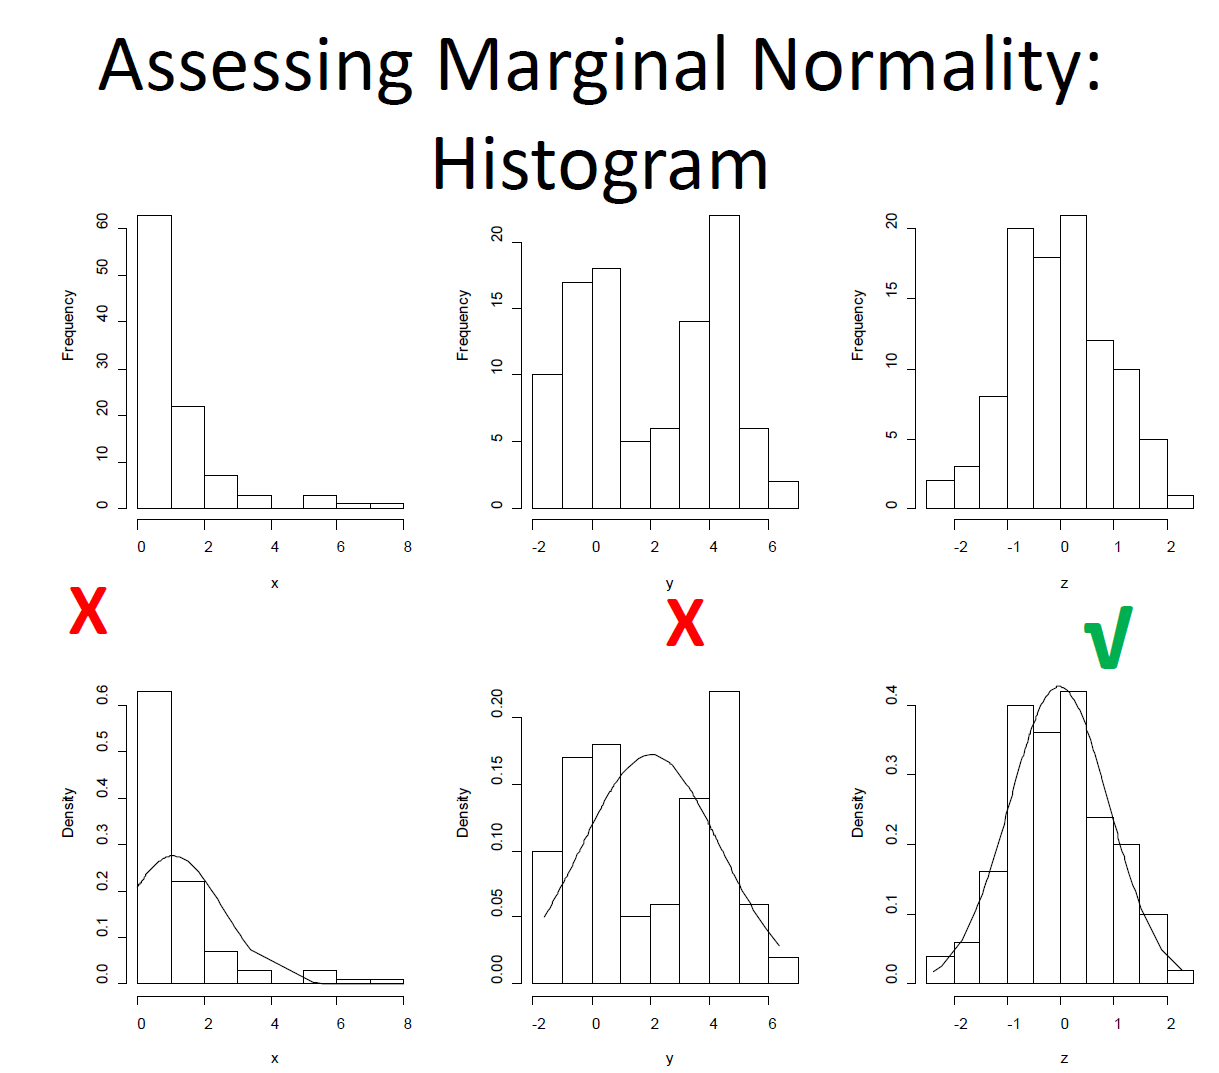
\includegraphics[width=0.6\linewidth]{img/assess_hist}
\end{frame}

\begin{frame}{QQ plots}
\protect\hypertarget{qq-plots}{}
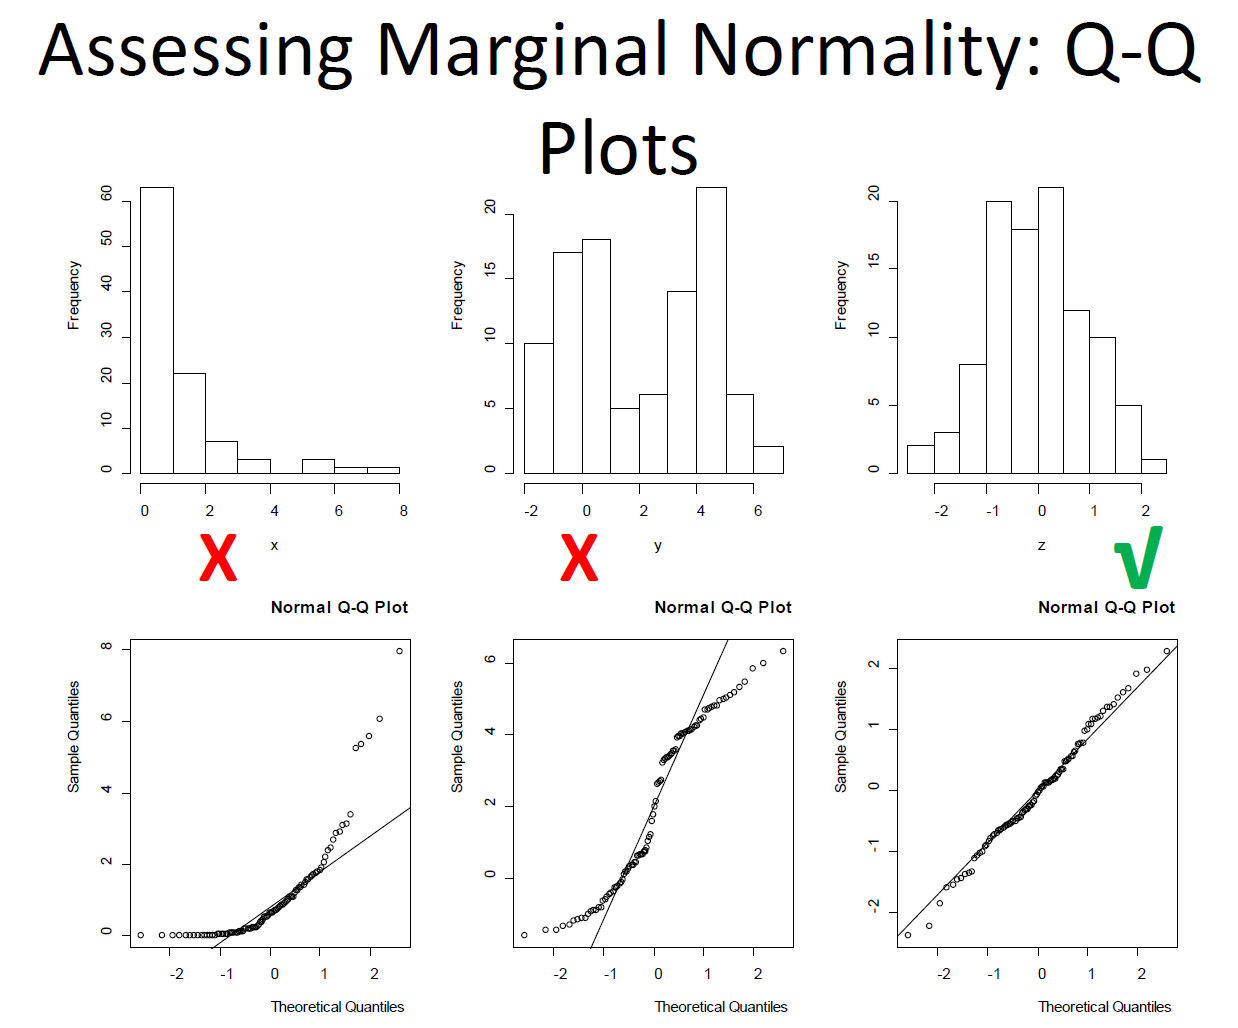
\includegraphics[width=0.6\linewidth]{img/assess_qq}
\end{frame}

\begin{frame}{Bivariate Scatter Plots}
\protect\hypertarget{bivariate-scatter-plots}{}
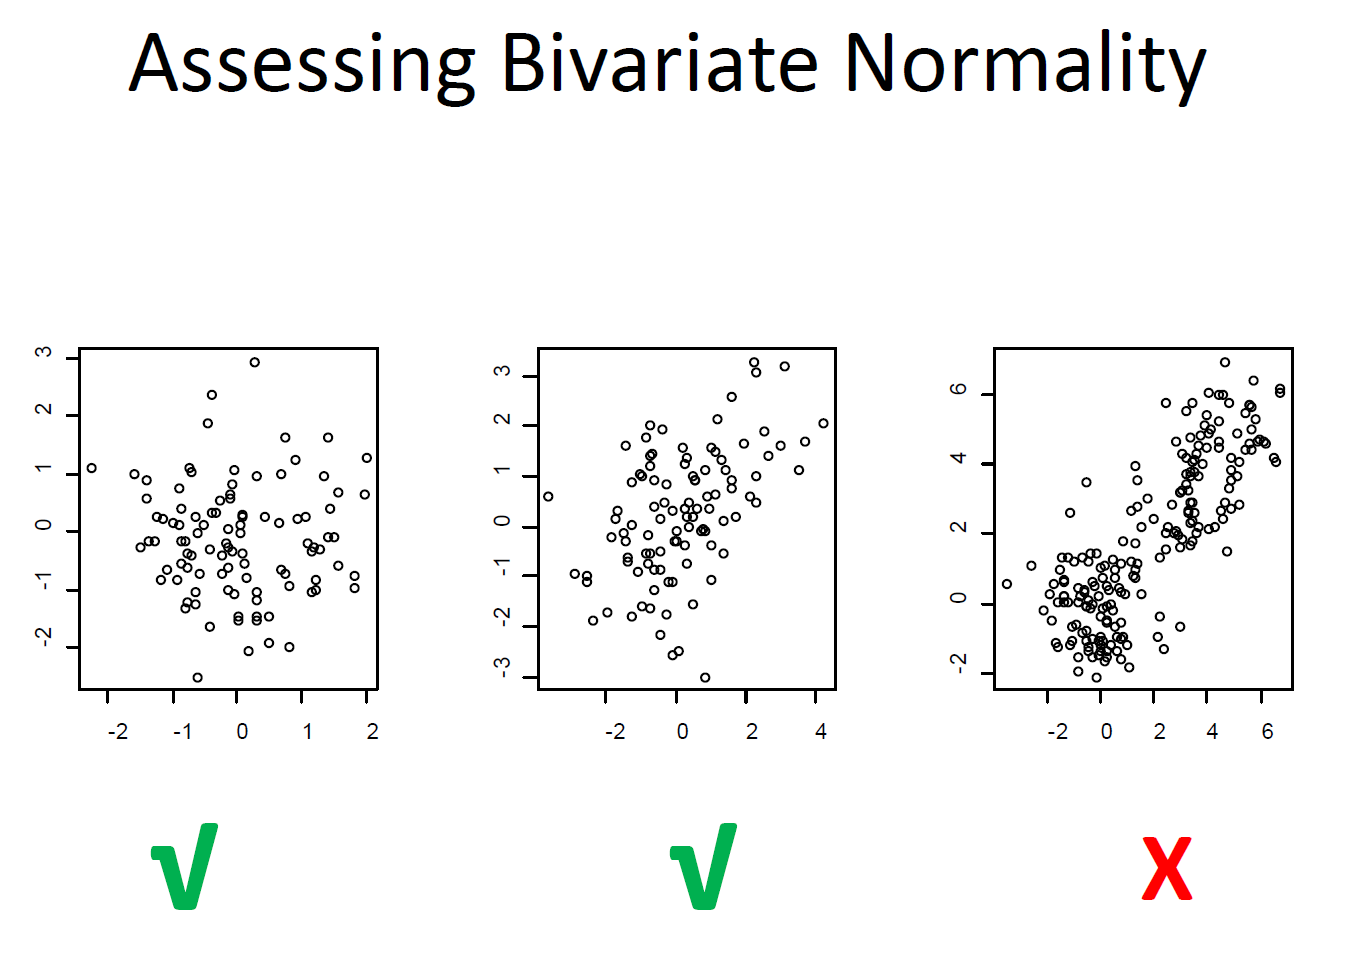
\includegraphics[width=0.6\linewidth]{img/assess_binorm}
\end{frame}

\begin{frame}{Large-Sample Results}
\protect\hypertarget{large-sample-results}{}
\begin{itemize}
\tightlist
\item
  Multivariate CLT
\end{itemize}

\[\begin{aligned}
& & \sqrt{n} (\bar{\mathbf X} -\boldsymbol \mu ) \overset{\mathbf D} \rightarrow N(\mathbf 0, \boldsymbol \Sigma)\\
& \Rightarrow & n(\bar{\mathbf X}-\boldsymbol \mu)^T \mathbf S^{-1}(\bar{\mathbf X}-\boldsymbol \mu) \rightarrow \chi_p^2
\end{aligned}
\]

\begin{itemize}
\tightlist
\item
  When \(n-p\) is large, we replace \(\frac{(n-1)p}{n-p}F_{p, n-p}\)
  with \(\chi_{p}^2\)
\item
  When \(n_1-p\) and \(n_2-p\) are large, we replace
  \(\frac{(n_1+n_2-2)p}{n_1+n_2-p-1}F_{p, n_1+n_2-p-1}\) with
  \(\chi_{p}^2\)
\end{itemize}
\end{frame}

\begin{frame}{Assignment 2: Due on Monday, May 1st}
\protect\hypertarget{assignment-2-due-on-monday-may-1st}{}
\tiny

\begin{itemize}
\item
  \textcolor{red}{Problem 1}: Choose a \(3-by-3\) covariance matrix with
  non-zero covariances. Also choose a sample size \(n\) (e.g., n=100,
  500, 1000, etc). Simulate 1,000 data sets from a trivariate normal
  distribution.

  \begin{enumerate}
  \setcounter{enumi}{-1}
  \tightlist
  \item
    Hints:
  \end{enumerate}

  \begin{itemize}
  \tightlist
  \item
    Hint 1: the R library MASS provides a function to generate a random
    sample from a multivariate normal distribution.
  \item
    Hint 2: Make sure that the covariance matrix you choose is positive
    definite. You can compute the eigenvalues by the ``eigen'' function
    in R and and check whether all the eigenvalues are positive.
  \end{itemize}

  \begin{enumerate}
  \tightlist
  \item
    Try to make sense of the covariance matrix by examining the pairwise
    scatter plots using the data you simulate.
  \item
    During the simulation, you will generate 1,000 Wishart distributed
    random matrices. Calculate the trace for each of them. Explain what
    distribution the traces should follow and examine their histogram.
  \end{enumerate}
\item
  \textcolor{red}{Problem 2}: Find a good data example to conduct a
  two-sample Hotelling's \(T^2\) test. Do not use the data example
  discussed in this course. Please (1) include visualizations as
  exploratory methods and (2) make conclusion in the context of the data
  example.
\item
  R Code should be included as appendices.
\end{itemize}

\normalsize
\end{frame}

\end{document}
